% Title icon: the Figure 2 prism, redrawn as vector art. Vertex positions and
% colors are sampled from readout_query_one_column_background.png so the icon
% matches the schematic; line widths are heavier than the source so the shape
% stays legible at ~2em height.
\documentclass[tikz,border=1pt]{standalone}
\begin{document}
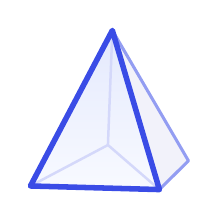
\begin{tikzpicture}[x=1pt,y=1pt]
  \definecolor{frontstroke}{RGB}{58,76,230}
  \definecolor{ghoststroke}{RGB}{147,157,242}
  \definecolor{ghostfill}{RGB}{242,242,250}
  \definecolor{fillupper}{RGB}{228,233,253}
  \definecolor{filllower}{RGB}{248,250,255}
  \definecolor{inneredge}{RGB}{212,216,250}
  \coordinate (T)  at (35.5,74.7);
  \coordinate (BL) at (5.9,18.5);
  \coordinate (BR) at (52.5,17.2);
  \coordinate (G)  at (63.0,27.6);
  \coordinate (C)  at (33.9,33.3);
  \fill[ghostfill] (T) -- (G) -- (BR) -- cycle;
  \draw[ghoststroke,line width=1.1pt,line join=round] (T) -- (G) -- (BR);
  \shade[top color=fillupper,bottom color=filllower] (T) -- (BL) -- (BR) -- cycle;
  \draw[inneredge,line width=0.9pt,line join=round]
    (C) -- (T) (C) -- (BL) (C) -- (BR);
  \draw[frontstroke,line width=2pt,line join=round] (T) -- (BL) -- (BR) -- cycle;
\end{tikzpicture}
\end{document}
